% Present the results for the original paper's RQs on the new data set.


%describe the setup of your experiment, e.g., the parameters of your model, how you split train-test, what are your baselines, evalution metrics, etc. 

In this section, we present the results of our empirical study with respect to our three research questions. For each research question, we present our motivation, approach, and results.
% \subsection{Experiment Setup}
\subsection{\rqone}
\label{sec:results:rq1}
\subsubsection{Motivation}
In this research question, we look to see whether there are any common characteristics of packages that release in-range breaking updates, and what types of updates end up breaking a client's build. In-range breaking updates are problematic for clients and finding common features of these updates is the first step in attempting to eliminate them.

\subsubsection{Approach}
We first wanted to see how the in-range breaking updates were distributed across different update types. Recall that semantic versioning splits updates into three primary categories: \textit{patch}, \textit{minor} and \textit{major} updates. On the breaking build issue reports, we extract the version the dependency was being updated from and the version the dependency was being updated to in order to determine whether the release was a major, minor, or patch update. We also want to compare how the number of in-range breaking updates by type compare to how often these update types are being released, as well as how often these update types are actually accepted by client version specifications.
\par
To determine what proportion each update type has of all releases, we examine all of the versions each of the dependency to determine how many patch, minor, and major updates the package has released. We determined what types of updates clients accept from providers by extracting each client's development and run-time dependency version specifications, and determining the type of updates they accept based on the rules outlined in Table \ref{tab:semver}.
\par
Another factor we investigate was whether the release frequency of provider packages tends to have any affect on how often they release in-range updates that break their clients. We tally the number of in-range updates each provider has that broke their client's, and compare the distributions across the total number of releases that package has, as well as the frequency at which that package releases new versions.

\subsubsection{Results}
We were able to extract the version ranges of the breaking dependency being updates for 63.77\% of the issue reports. This is because Greenkeeper will bundle upgrades for the packages that have to be upgraded together, and if one of the updates in the bundle breaks the client's build, the issue report is opened for all of the updates in the bundle. We are not able to determine the specific breaking dependency in the bundle, and we therefore omit these issue reports from our analysis.
\par
We found that 65.15\%, 34.69\%, and 0.16\% of in-range breaking updates are patch, minor, and major updates, respectively. These results would suggest that package developers are not following the semantic versioning scheme, which states that only major updates should be used to signify a breaking change in the package. However, patch and minor updates occur much more frequently than major updates. We found that 64.37\%, 28.25\%, and 7.37\% of package releases were patch, minor and major updates, respectively. This explains to some degree why the number of in-range breaking updates that are patch and minor updates is larger than major updates, since patch and minor updates occur more frequently then major updates.
\par
Additionally, we found that major updates are far less likely to be accepted as in-range updates by clients. Recall that, in order for an update to be considered in-range, the client must specify the range of updates they are willing to accept. We found that 12.53\% of dependencies are pinned by clients, which means the provider will never be able to release an in-range update. Of the remaining dependencies, 3.74\%, 82.31\%, and 1.08\% are accepting patch, minor, and major updates, respectively, which would further reduce the number of major updates that are considered to be in-range for clients. These results are summarized in Figure \ref{fig:bar_stacked_breaks_releases_accepted_update_types}
\begin{figure}[h]
    \centering
    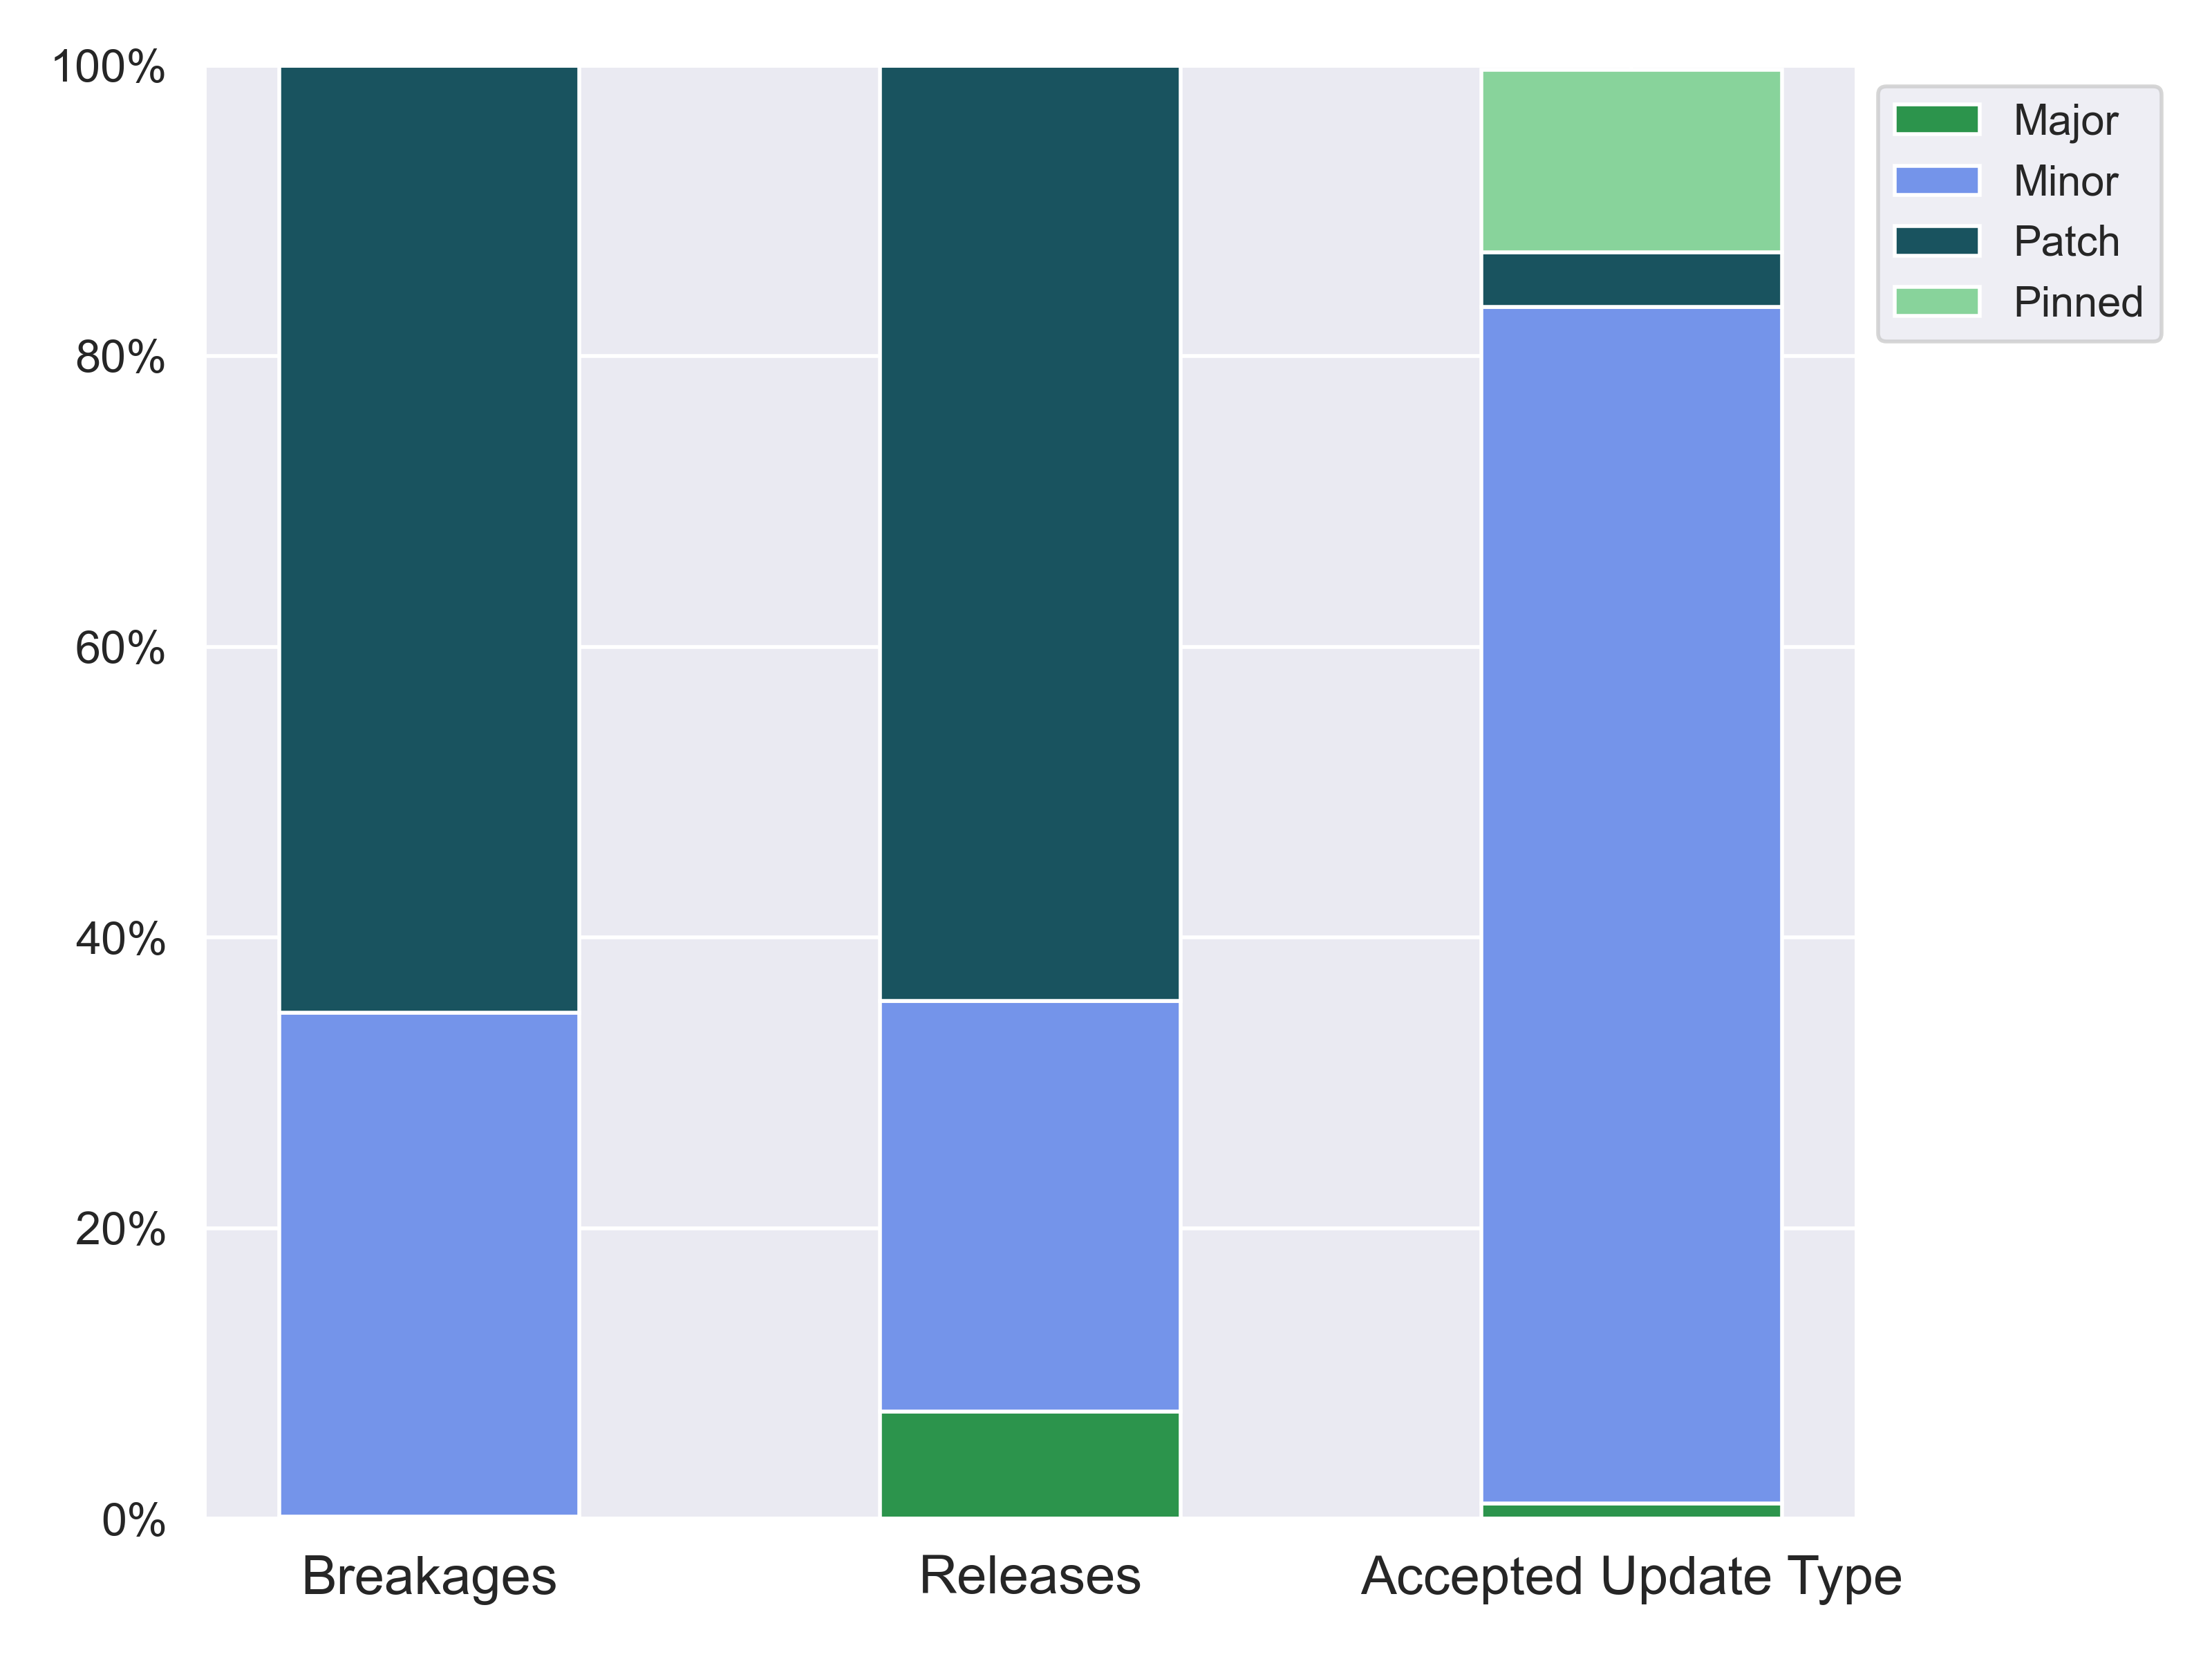
\includegraphics[width=\linewidth]{images/rq1_stacked.png}
    \caption{Distribution of update types for in-range breakages, package releases, and accepted update types}
    \label{fig:bar_stacked_breaks_releases_accepted_update_types}
\end{figure}
\par
In terms of how the release practices of packages affect how often they release in-range breaking updates, we found that the number of broken builds increases by 0.07 for every additional release a package makes. Intuitively, this result is expected. The more releases a package has, the more opportunities there are that a release will break a client's build. We also look at the distribution of build breakages caused by a provider against the frequency at which they release new versions. We found that the number of in-range breakages decrease by $3.7e-10$ as the release frequency increases, which is not strong evidence that a higher release frequency is less likely to cause in-range breaking updates, or vice versa. These results are visualized in Figure \ref{fig:dist_breaks_to_package_release_total_and_freq}.
\begin{figure*}[h]
    \centering
    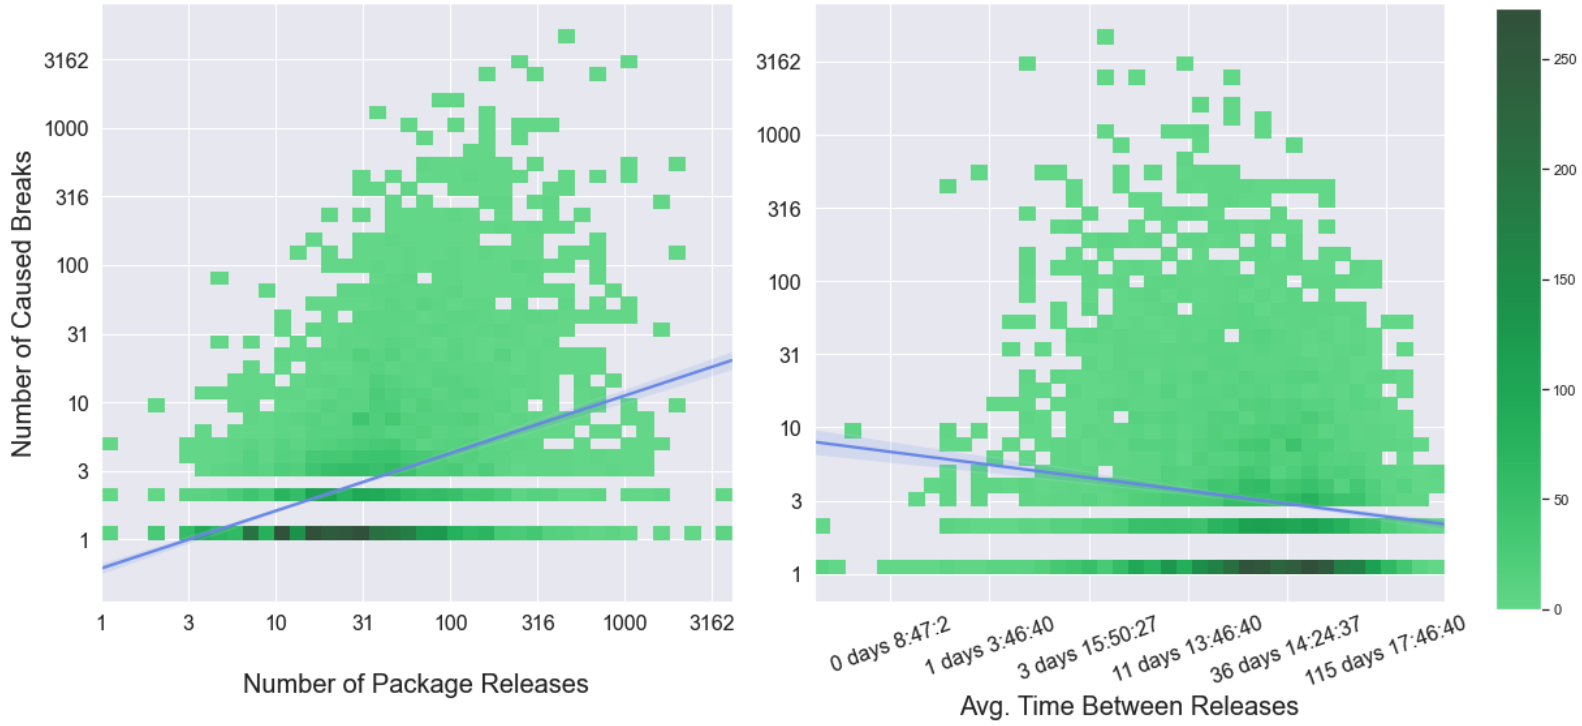
\includegraphics[width=15cm]{images/breakages_to_package_releases_and_frequency_manual.png}
    \caption{Distribution of number of cause breakages and total package releases (left) and release frequency (right)}
    \label{fig:dist_breaks_to_package_release_total_and_freq}
\end{figure*}
\newline
\par
\fbox{%
    \parbox{8cm}{%
        While the majority of clients will accept minor updates, most breakages are caused by patch updates. Packages with higher total and more frequent releases tend to cause more breakages.
    }%
}
\subsection{\rqtwo}
\label{sec:results:rq2}
\subsubsection{Motivation}
As previously mentioned, in-range breaking updates should be treated with a sense of urgency by client developers, as any attempt by users to install their package after the in-range dependency update will fail. In this research question, we look at how client developers respond to these in-range updates, and what actions they have to take in order to resolve their build.

\subsubsection{Approach}
To answer this research question, we examine a number of attributes related to the in-range breaking build issue reports opened in the client projects. We look at the content of the issue reports themselves, the comments on the issue reports, as well as the types of changes that are made by developers in order to fix their builds, Additionally, we look at the effectiveness of Greenkeeper's automatic attempts at pinning the breaking dependency as a first attempt to resolve the client's build.

\subsubsection{Results}
We found that 79.82\% of in-range breaking update issue reports were eventually closed, with a median time to close the issue of 4 days and 11 hours. We examine the comments on in-range breaking build issue reports in order to gain insight into how clients are responding to these issues. We found that 85.93\% of issues have at least 1 comment. This is expected, as Greenkeeper will attempt to pin the breaking dependency immediately after opening the majority of issue reports, and will automatically comment the build result of pinning the dependency on the issue report. 47.95\% of issues have at least 2 comments. We hypothesised that approximately half of all comments on the issue reports were from users. However, further analysis revealed that only 2.93\% of comments were from non-bot users on GitHub, and that 96.89\% of all comments are from the Greenkeeper bot itself, with the remaining comments being from other bots.
\par
Specifically examining the user comments, we found that the median response time was 2 days and 12 hours. We classified these comments using regular expressions to match specific phrases and patterns. We found that users are specifically referencing a fix for the issue 34.5\% of the time, while the simply mention the issue has been fixed 17.4\% of the time. 18.3\% of comments indicate the build failure is a false alarm, referencing a flaky test, CI hiccup, or that they simply re-ran the build pipeline and it passed without incident. The proportion of user comment types, as well as the average response times for each type are summarized in Figure \ref{fig:issue_comments}
\begin{figure*}[h]
    \centering
    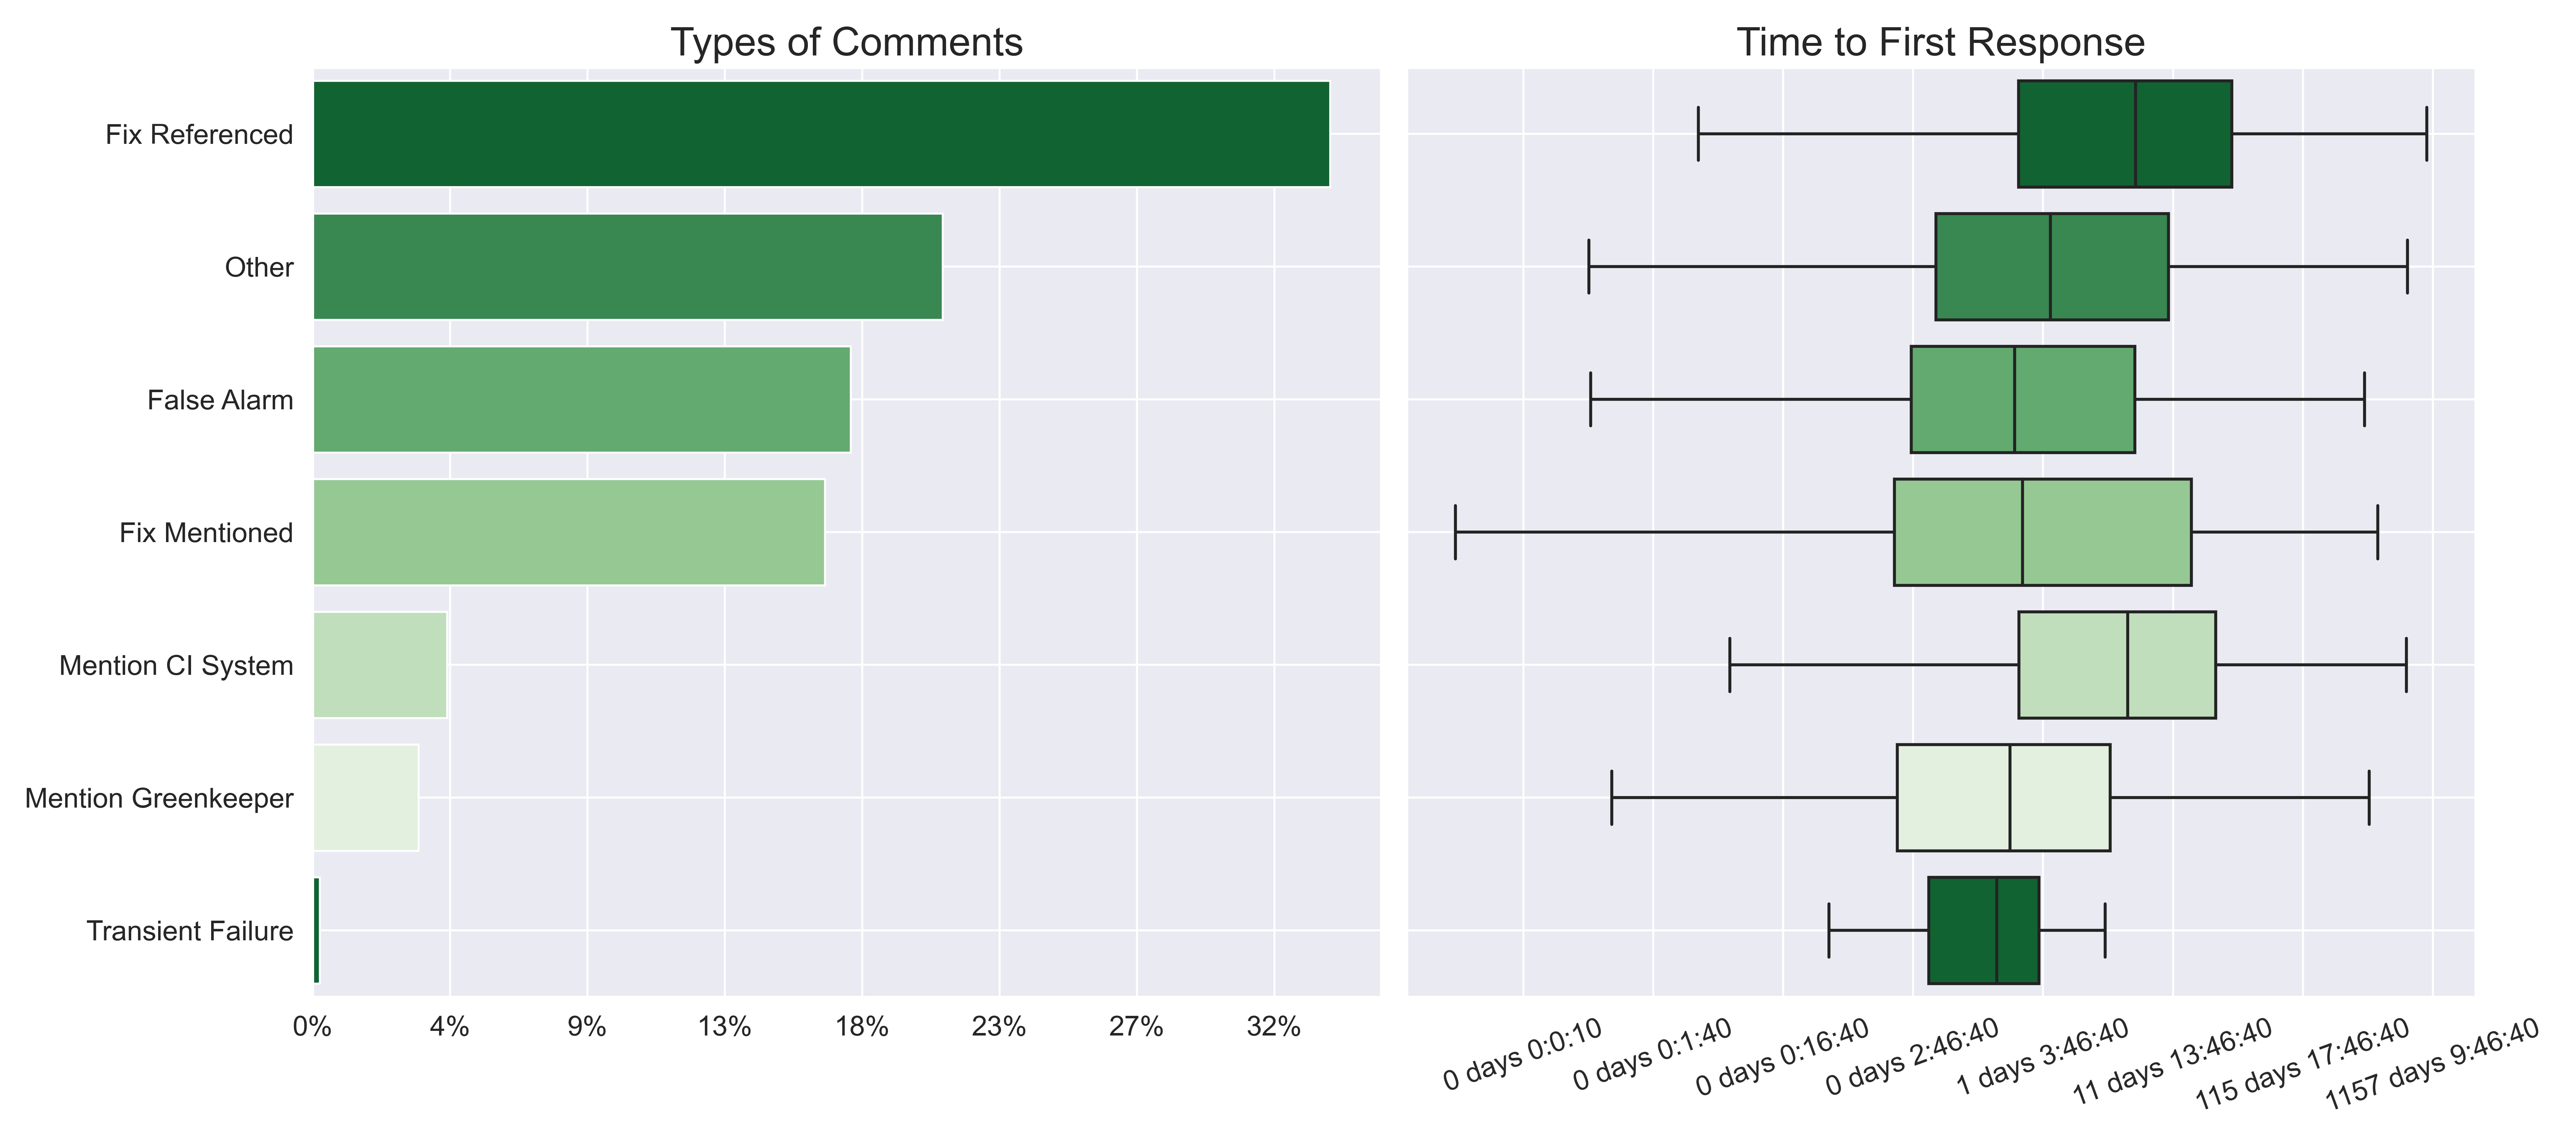
\includegraphics[width=16cm]{images/types_of_comments_and_time_until_comment_type.png}
    \caption{Most common types of comments left by users on in-range breaking build issue reports (left) and how long users take to make each response (right) }
    \label{fig:issue_comments}
\end{figure*}
\par
We saw that practitioners were referencing fixes on these issue reports, so we investigated what these fixes entail. We found that 69.7\% of referenced commits include changes the \textit{package.json} file, 28.5\% include changes to the \textit{package-lock.json} file, and 25.6\% include changes to the \textit{yarn.lock} file. These are all files that are used to specify a projects dependencies. The two lock files are automatically generated and so have a relatively high commit churn, with the \textit{package-lock.json} file having a median commit churn of 101 additions and 130 deletions, and the \textit{yarn.lock} having a median commit churn of 44 additions and 59.5 deletions. However, the \textit{package.json} file, which is manually maintained, has a median commit churn of 1 addition and 1 deletion per commit when fixing an in-range breaking build issue. This suggests that, in order to fix their build, users are simply updating their accepted dependency version range, such as pinning the dependency that is failing the build. Figure \ref{fig:changed_files} summarized the most common files changed in referenced commits on in-range breaking build issues, as well as their commit churn. Additionally, these results shows that it is uncommon for clients to modify their source code that uses these dependencies in order to fix their builds.
\begin{figure*}[h]
    \centering
    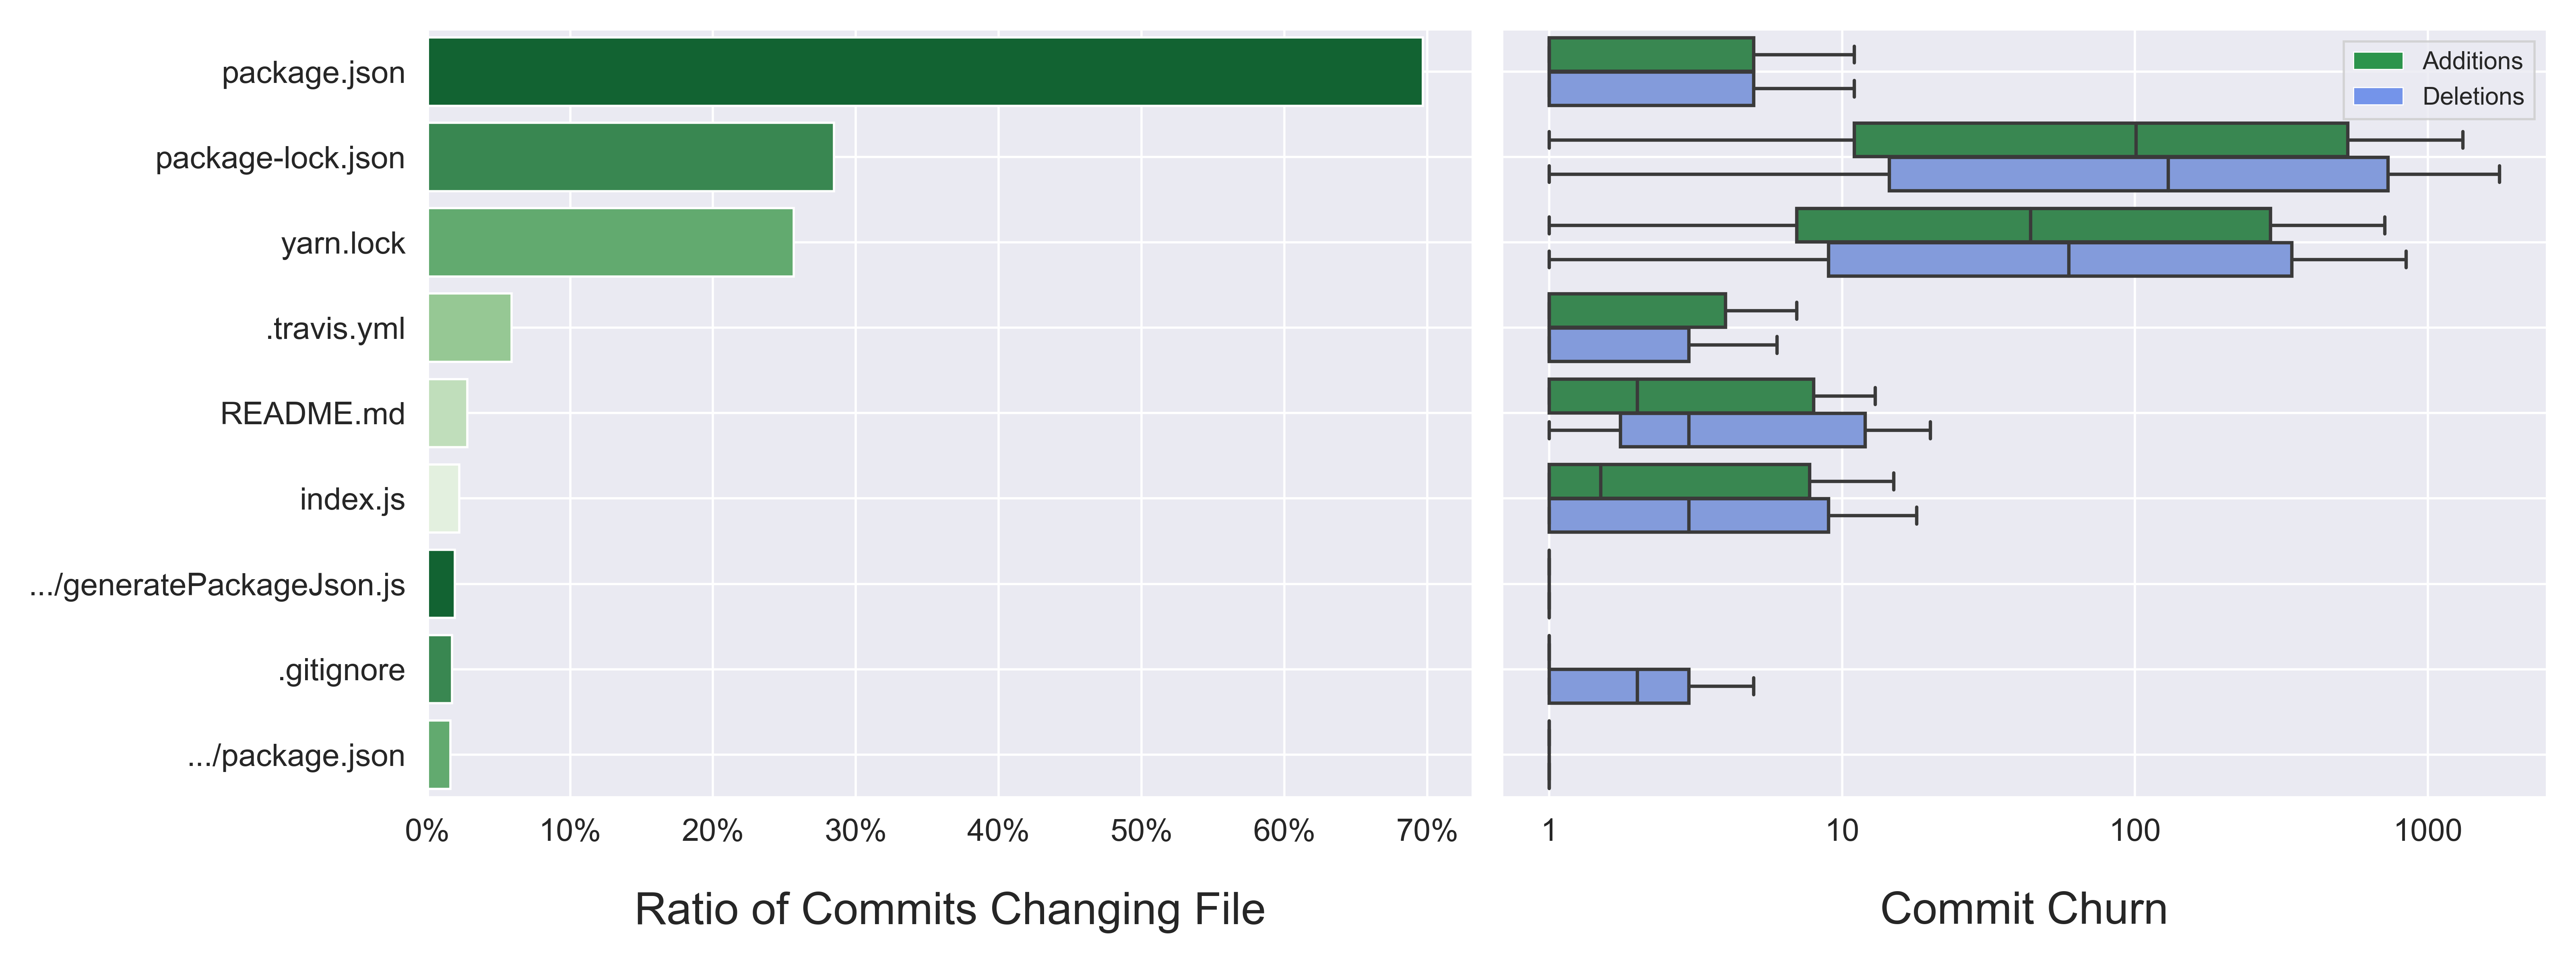
\includegraphics[width=\linewidth]{images/changed_files_ratio_and_commit_churn.png}
    \caption{Most common files changed in commits referenced by in-range breaking build issue reports (left) and the commit churn of each file (right)}
    \label{fig:changed_files}
\end{figure*}
\par
When the Greenkeeper bot opens a breaking build issue report, it will automatically attempt to pin the dependency to the previous version and re-run the build to determine if the issue can be resolved. Pinning a dependency is a legitimate option when developers don’t have the time or resources to fix a problem introduced by a dependency update. Greenkeeper will bundle upgrades for the packages that have to be upgraded together, and it won’t attempt to pin all of the packages in the bundle, which is why 28.1\% of issues don’t have a pin attempt. However, of the issue reports that did have a pin attempt, only 33.1\% resulted in the client's build passing again. This indicates that the majority of these in-range breaking build update issue reports are not actually caused by the dependency being updated. In order to better understand the reasons as to why so many pin attempts fail, we manually analyze a sample of the issue reports that have a failed pin attempt. We found that clients improperly configuring their projects build pipeline was the primary reason for the dependency updates failing, including missing configuration files, invalid credentials, or inconsistent environment versions. We also saw that the builds can fail due to flaky tests, request timeouts, and even  attempting to run the build before the branch had been created in the project repository.
\par
Additionally, we found that Greenkeeper does not take into account the type of error that occurs in the pipeline when testing new dependency updates, and will consider any error that occurs in the pipeline as a build failure. This means that, for example, if a developer that does not conform to the project's linter configuration, then all subsequent builds will fail, and Greenkeeper will open in-range breaking update issue reports for any dependencies that release a new in-range version. If the dependency continues to release new versions, the issue report will become flooded with comments from Greenkeeper confirming that the build is still failing, introducing a lot of noise into projects and distracting from valid issue reports, which practitioners say is one of the main reasons for not using automated dependency management tools \cite{ACM2017_Mirhosseini_AutomatedPullRequests}.
\newline
\par
\fbox{%
    \parbox{8cm}{%
        The majority of client responses mention a fix or confirm the issue is invalid. Most fixes involve small changes to dependency specification files. While pinning the dependency is a legitimate option, it is not as successful as expected due to builds failing for reasons not related to the dependency being updated.
    }%
}
\subsection{\rqthree}
\label{sec:results:rq3}
\subsubsection{Motivation}
In the previous research question, we looked at how clients respond to in-range breaking updates. However, while it is the client's build that is failing, the root cause of the issue could originate from the provider. In this research question, we look to see whether in-range breaking updates prompt a response from the provider packages.
\subsubsection{Approach}
Initially, we examined all of the comments made by users on the in-range breaking build issue reports looking for potential references to issue report made in the dependency package that were related to the client's breaking build issue report. We were not successful in finding any, so we took a different approach. We hypothesis that, if a release from a package provider causes an in-range breaking builds in a high proportion of client, the next release the provider package makes would happen quicker than usual. To test this, we compare the average release frequency of packages against the time it takes a package to release the next update immediately following an update that causes an in-range breaking build in at least 20\% of clients that depend on it.
\par
First, we determine the number of clients that are using each of the provider packages we have release information on in our data set. We then determine how many issue reports were opened for each release made by each provider package. Using this information, we determine the ratio of in-range breaking update issue reports that each release made by every provider package caused. This allows us to categorize each release either as a breaking release or a non-breaking release. We then compare the release frequency of the non-breaking releases to the time to the release immediately following each breaking release.

\subsubsection{Results}
We first used all release records in our analysis including releases that did not cause any in-range update breaking issues in any clients. We found that the median release time after non-breaking releases was 1 day and 22 hours (IQR = 3 hours - 10 days 12 hours), while the median release time immediately following a breaking release was 8 days and 6 hours (IQR = 1 day and 3 hours - 39 days and 6 hours). From these results, it appears that the release that immediately follow an update that breaks a proportion of clients tends to take longer to be made available. However, we choose to perform further analysis on only breaking releases.
\par
We examine only the set of releases that caused at least one in-range breaking build issue report to be opened in a client. While all these releases caused at least one breaking build, we still classify a breaking release as a release that caused at least 20\% of the package's client's builds to break. The median release time immediately following a breaking release was still 8 days and 6 hours (IQR = 1 day and 3 hours - 39 days and 6 hours), as that data set was unaffected, but the median release time after non-breaking releases was 8 days and 6 hours (IQR = 1 day 3 hours - 39 days 6 hours). These results can be seen in Figure \ref{fig:time_until_next_breaking_release}.
\begin{figure*}[h]
    \centering
    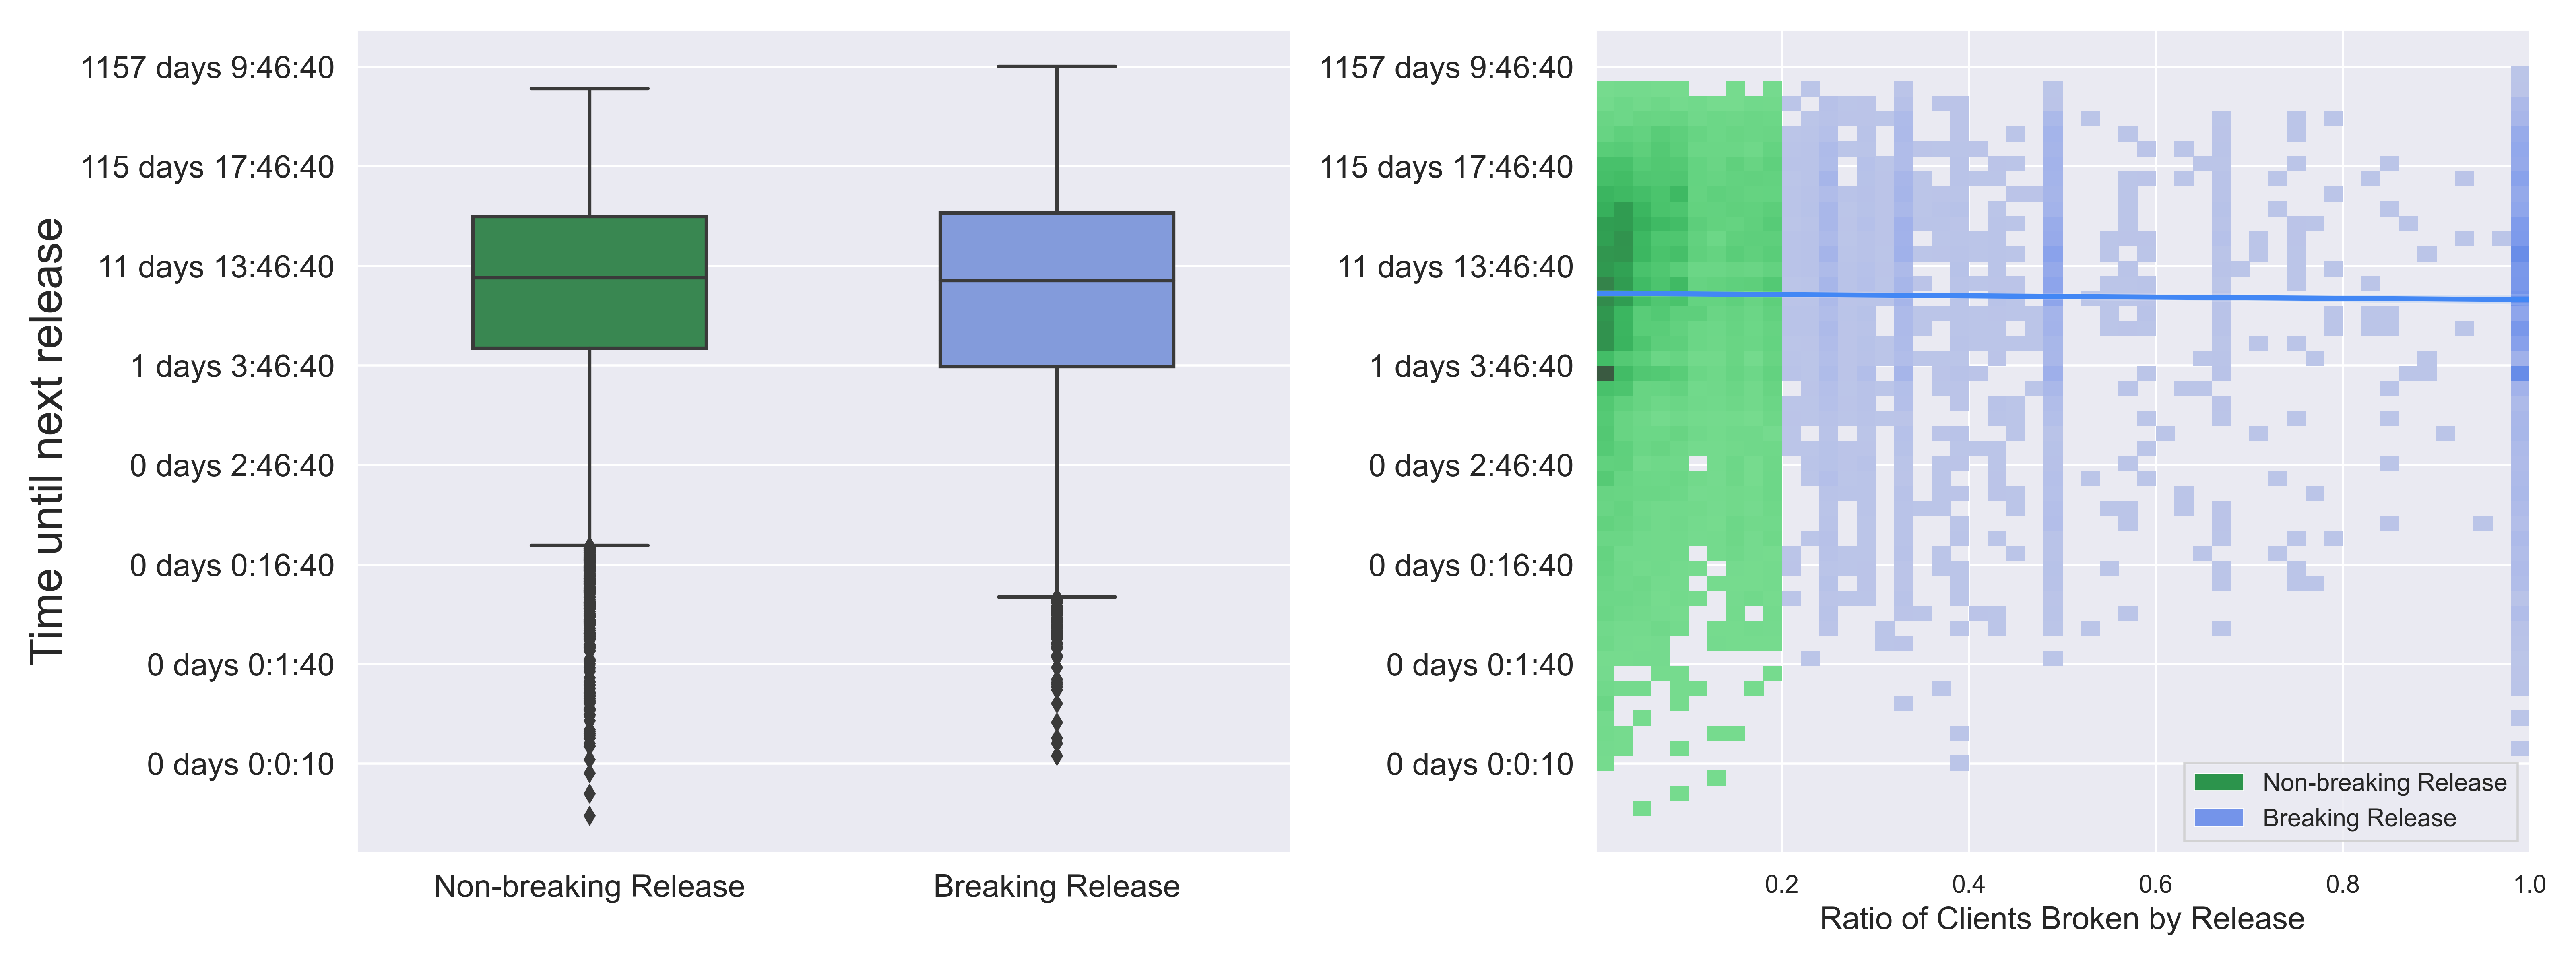
\includegraphics[width=\linewidth]{images/time_until_next_release_after_break_plots.png}
    \caption{Time until next release for non-breaking and breaking releases}
    \label{fig:time_until_next_breaking_release}
\end{figure*}
\newline
\par
\fbox{%
    \parbox{8cm}{%
        We did not find any indication that client's are filing issue reports with provider packages that release in-range breaking updates. There is no statistical difference that indicates that breaking releases are immediately followed up by a quicker release than normal.
    }%
}
